\documentclass{beamer}
\usepackage[T1]{fontenc}
\usepackage[latin1]{inputenc}
\usepackage[frenchb]{babel}
\usepackage{graphicx}
\usepackage{subfig}

\graphicspath{{Images/}}

\usetheme{Hannover}

\beamertemplatenavigationsymbolsempty

\definecolor{bleufonce}{rgb}{0.1,0.1,0.8}
\definecolor{grisbleu}{rgb}{0.8,0.8,0.9}
\definecolor{rougefonce}{rgb}{0.8,0.1,0.1}
\definecolor{grisrouge}{rgb}{0.9,0.8,0.8}
\definecolor{vertfonce}{rgb}{0.1,0.8,0.1}
\definecolor{grisvert}{rgb}{0.8,0.9,0.8}
\definecolor{bleuunistra}{RGB}{15,80,150}
\setbeamercolor{palette quaternary}{fg=white,bg=bleuunistra}
\setbeamercolor{titlelike}{parent=palette quaternary}

\setbeamertemplate{blocks}[rounded][shadow=true] 
\setbeamercolor{block title}{bg=bleufonce,fg=white}
\setbeamercolor{block body}{bg=grisbleu}
\setbeamercolor{block title alerted}{bg=rougefonce,fg=white}
\setbeamercolor{block body alerted}{bg=grisrouge}
\setbeamercolor{block title example}{bg=vertfonce,fg=white}
\setbeamercolor{block body example}{bg=grisvert}

\title[Projet El\'ements Finis]{R\'esolution d'un probl\`eme aux valeurs propres de l'op\'erateur rotationnel.}
\subtitle{R\'eseaux, M2 CSMI}

\author{Romain HILD\\J\'er\^ome SPECHT}
\institute{Universit\'e de Strasbourg}

\begin{document}

\begin{frame}

\includegraphics[scale=0.2]{uds.jpg}
\includegraphics[scale=0.15]{po.jpg}
\titlepage
\end{frame}

\begin{frame}{Contexte}
\begin{block}{Plastic Omnium}
\begin{itemize}
\item Leader de son domaine
\item Cherche \`a \^etre en avance sur les probl\`emes futurs.
\item Diminution de l'\'emission du $C0_2$.
\end{itemize}
\end{block}
\begin{eqnarray}
\label{pb}
\left\{
\begin{aligned}
&\frac{\partial v}{\partial t} + (curl\  v)\times v + \nabla p -\frac{1}{Re}curl^2\  v-f = 0\\
&div\ v = 0\\
&v\big\rvert_{t=0} = v_0\\
&v\cdot n\big\rvert_{\partial\Omega} = \alpha_0\\
&(curl\  v)\cdot n\big\rvert_{\partial\Omega} = \alpha_1\\
&(curl^2\  v)\cdot n\big\rvert_{\partial\Omega} = \alpha_2
\end{aligned}
\right.
\end{eqnarray}
\end{frame}

\begin{frame}{Probl\`eme}
\begin{block}{R\'esolution du probl\`eme (\ref{pb})}
\begin{itemize}
\item R\'esolution directe trop lente,
\item S\'eparation du probl\`eme en espace de celui en temps,
\item Utilisation des fonctions propres de l'op\'erateur rotationnel pour exprimer la vitesse,
\item On cherche \`a r\'esoudre (\ref{vp}).
\end{itemize}
\end{block}
\begin{eqnarray}
\label{vp}
(\lambda_i,g_i)\in\mathbb{R}\times D^1(\Omega)\quad \left\{
\begin{aligned}
&curl^2\  g_i = \lambda_i g_i\\
&g_i\cdot n\big\rvert_{\partial\Omega} = 0\\
&curl\  g_i\cdot n\big\rvert_{\partial\Omega} = 0\\
&curl^2\  g_i\cdot n\big\rvert_{\partial\Omega} = 0
\end{aligned}
\right.
\end{eqnarray}
\end{frame}

\begin{frame}{Forme variationnelle}
On obtient la forme suivante en multipliant par $\varphi$ ($\varphi=\varphi_0+\nabla\phi$ et $\varphi\big\rvert_{\partial\Omega} = \nabla\phi$) et en int\'egrant :
\[
\int_\Omega curl^2\ g\cdot\varphi\ dX = \int_\Omega\lambda g\cdot \varphi\ dX
\]
Puis en int\'egrant par partie :
\[
\int_\Omega curl\ g\cdot curl\ \varphi\ dX +�\int_{\partial\Omega} (curl\ g\times \nabla\phi)\cdot n\ d\Gamma = \lambda\int_\Omega g\cdot \varphi\ dX
\]
En utilisant le th\'eor\`eme de Green-Ostrogradski et en d\'eveloppant la divergence :
\[
\begin{aligned}
\int_\Omega curl\ g\cdot curl\ \varphi\ dX &+�\int_\Omega \nabla\phi\cdot curl^2\ g\ dX\\ 
&-\int_\Omega curl\ g\cdot curl\ \nabla\phi\ dX  = \lambda\int_\Omega g\cdot \varphi\ dX
\end{aligned}
\]
\end{frame}

\begin{frame}{Forme variationnelle}
En int\'egrant par partie le deuxi\`eme terme :
\[
\begin{aligned}
\int_\Omega curl\ g\cdot curl\ \varphi\ dX &+�\int_{\partial\Omega} \phi(curl^2\ g\cdot n)\ d\Gamma \\
&- \int_\Omega \phi(div(curl^2\ g))\ dX  = \lambda\int_\Omega g\cdot \varphi\ dX
\end{aligned}
\]
Ce qui am\`ene \`a :
\begin{eqnarray}
\int_\Omega curl\ g\cdot curl\ \varphi\ dX = \lambda\int_\Omega g\cdot \varphi\ dX
\end{eqnarray}
\end{frame}

\begin{frame}{Des r\'esultats}
\begin{figure}[H]
	\makebox[\textwidth][c]{
		\subfloat[mode00]{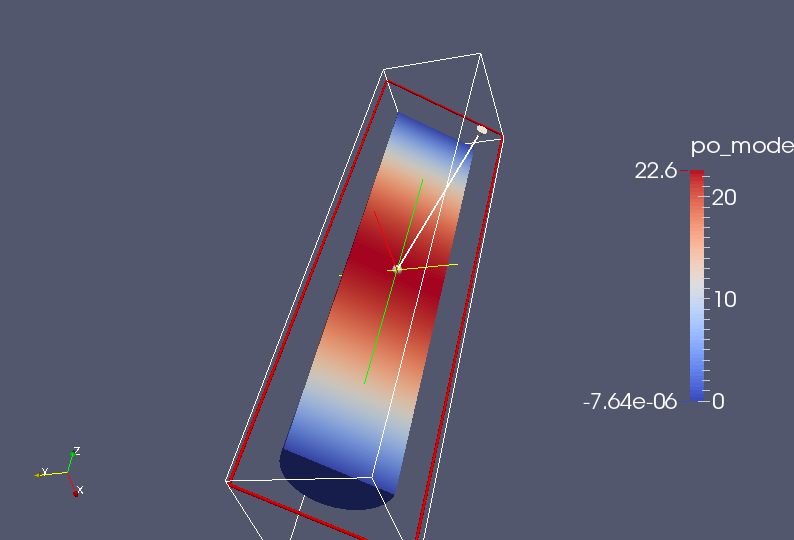
\includegraphics[scale=0.15]{mode00}}\ 
		\subfloat[mode19]{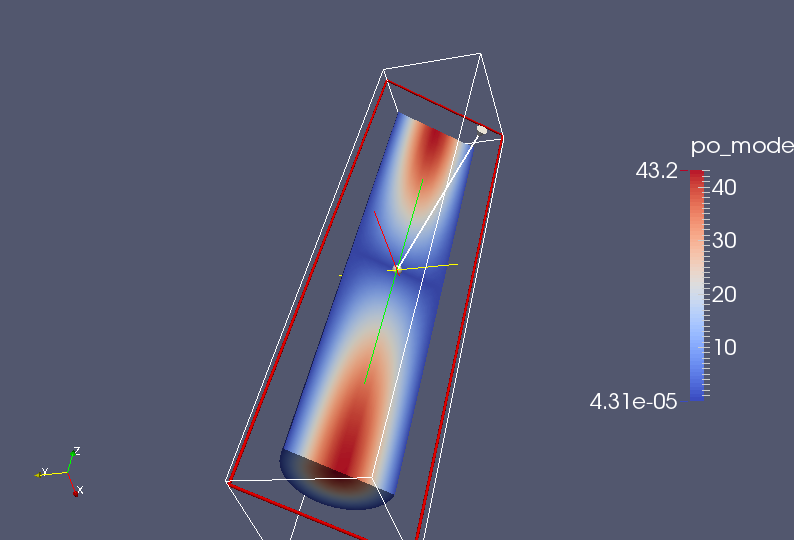
\includegraphics[scale=0.15]{mode19}}
	}\\
	\makebox[\textwidth][c]{
		\subfloat[mode57]{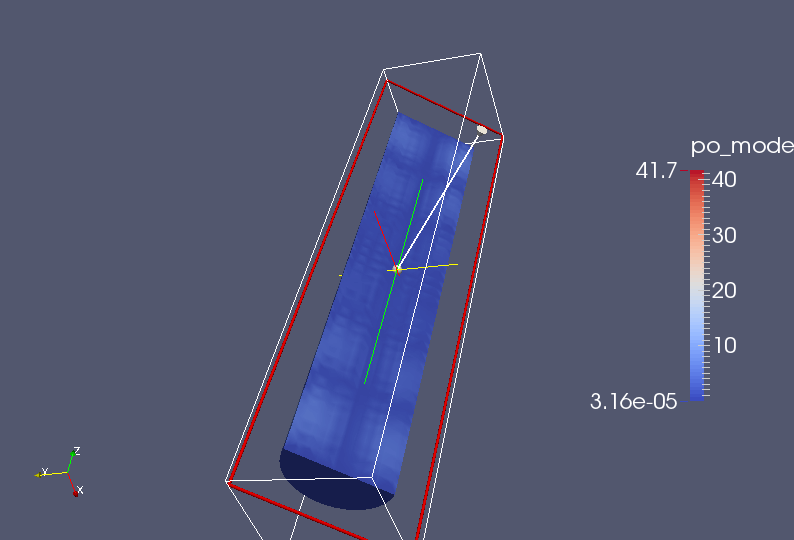
\includegraphics[scale=0.15]{mode57}}\ 
		\subfloat[mode194]{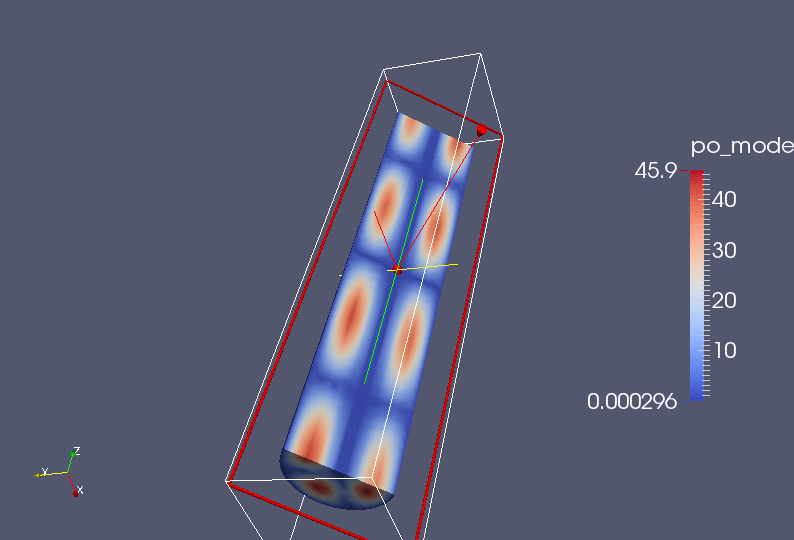
\includegraphics[scale=0.15]{mode194}}
	}
	\caption{composant z des fonctions propres}
	\label{resultats}
\end{figure}
\end{frame}

\begin{frame}{Des r\'esultats}
\begin{figure}[H]
\makebox[\textwidth][c]{
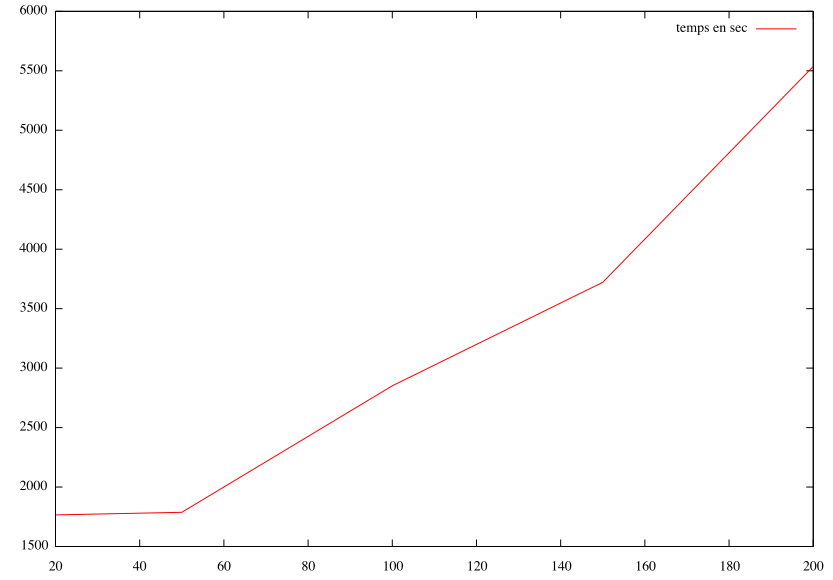
\includegraphics[scale=0.3]{temps_mode}}
\caption{Temps de calcul pour 10 processeurs avec 20, 50, 100, 150 et 200 modes}
\label{temps_proc}
\end{figure}
\end{frame}

\begin{frame}{Conclusion}
\begin{block}{Un projet inachev\'e}
\begin{itemize}
\item Probl\`eme dans le programme.
\item Pivot nul.
\item Temps de calcul en fonction du nombre de processeurs incoh\'erent.
\item Il reste encore beaucoup \`a faire.
\end{itemize}
\end{block}
\center
Merci de votre attention.
\end{frame}




\end{document}
